\section{Draw}
$draw(f,x)$ draws a graph of the function $f$ of $x$.
The second argument can be omitted when the dependent variable
is literally $x$ or $t$.
The vectors $xrange$ and $yrange$ control the scale of the graph.

\medskip
\verb$draw(x^2)$

\medskip
\begin{center}
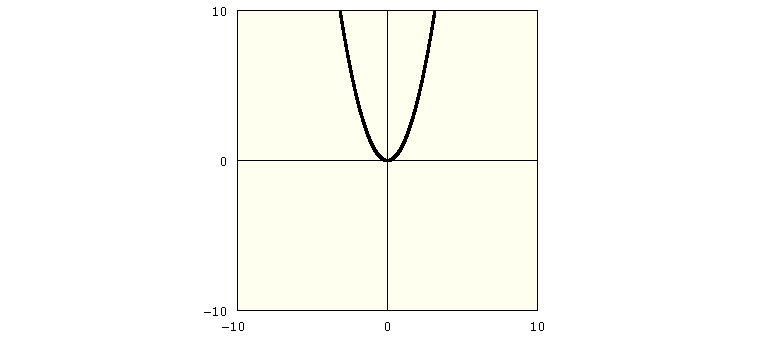
\includegraphics[scale=0.4]{parabola.png}
\end{center}

\verb$xrange=(-1,1)$

\verb$yrange=(0,2)$

\verb$draw(x^2)$

\medskip
\begin{center}
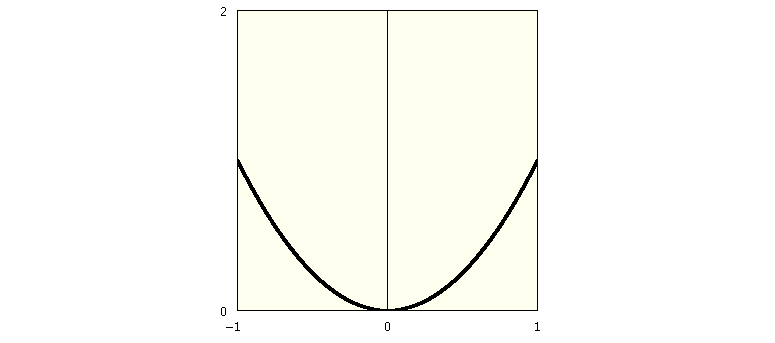
\includegraphics[scale=0.4]{parabola2.png}
\end{center}

\verb$clear$

\medskip
\noindent
The clear command (or a click of the Clear button)
resets $xrange$ and $yrange$.
This needs to be done so that the next graph
appears as shown.

\newpage

\noindent
Parametric drawing occurs when a function returns a vector.
The vector $trange$ controls the parameter range.
The default range is $(-\pi,\pi)$.

\medskip
\verb$f=(cos(t),sin(t))$

\verb$draw(5*f)$

\medskip
\begin{center}
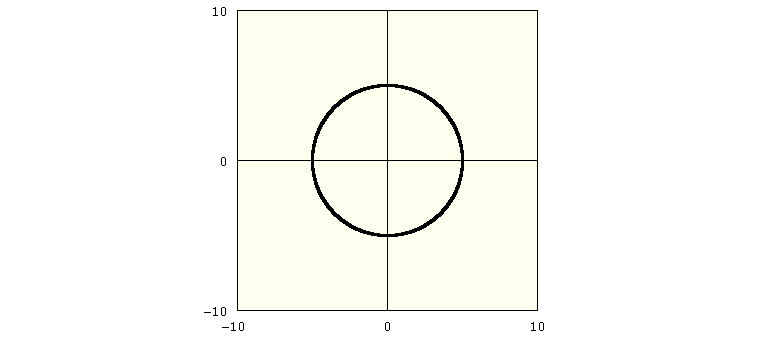
\includegraphics[scale=0.4]{circle.png}
\end{center}

\verb$trange=(0,pi/2)$

\verb$draw(5*f)$

\medskip
\begin{center}
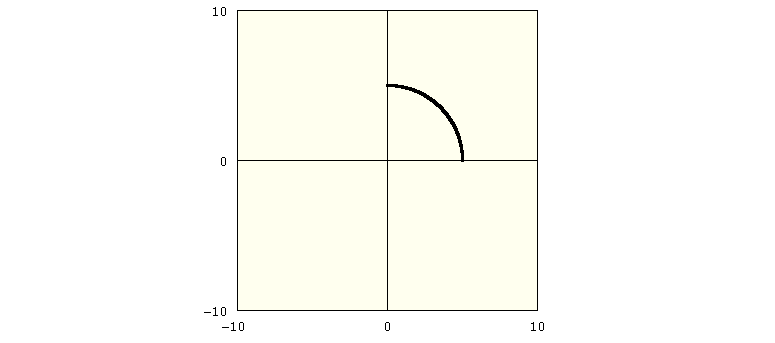
\includegraphics[scale=0.4]{circle2.png}
\end{center}

\newpage

\noindent
Here are a couple of interesting curves and the code for drawing them.
First is a lemniscate.

\medskip
\verb$clear$

\verb$X=cos(t)/(1+sin(t)^2)$

\verb$Y=sin(t)*cos(t)/(1+sin(t)^2)$

\verb$draw(5*(X,Y))$

\medskip
\begin{center}
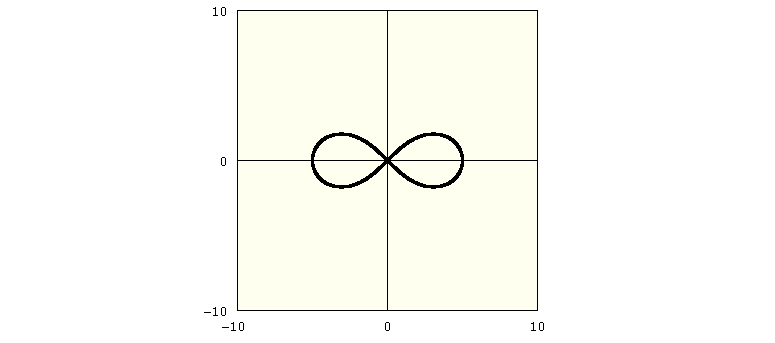
\includegraphics[scale=0.4]{lemniscate.png}
\end{center}

\medskip
\noindent
Next is a cardioid.

\medskip
\verb$r=(1+cos(t))/2$

\verb$u=(cos(t),sin(t))$

\verb$xrange=(-1,1)$

\verb$yrange=(-1,1)$

\verb$draw(r*u)$

\medskip
\begin{center}
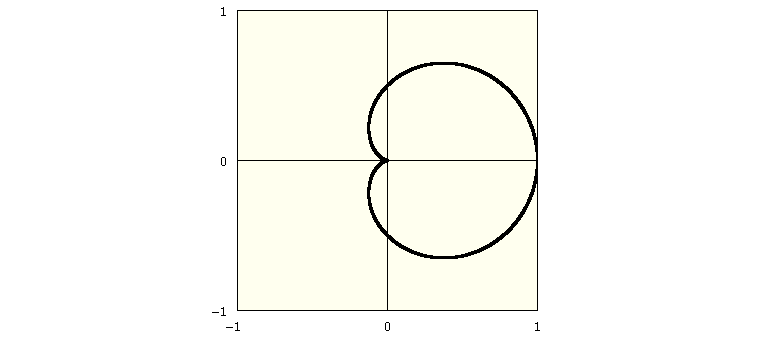
\includegraphics[scale=0.4]{cardioid.png}
\end{center}

